\section{Módulos}
\subsection {Rotinas}
\subsubsection{Multiplexação no tempo}
Para tratar indisponibilidade dos módulos devido a tentativas de reconexão e conexão e requisições não-gerenciadas, e, assim, aumentar a disponibilidade, existem além do circuito antitravamento e \textit{hard reset} diversas rotinas de tratamento. Elas contemplam desde configuração inicial, reconfigurações, coletas de dados e atuação por meio de relés até conexão, desconexão, reconexão e envio de dados. Elas foram multiplexadas no tempo da seguinte forma:

\begin{figure} [H]
	\centering
	\caption{Rotina de multiplexação de procedimentos no tempo}
  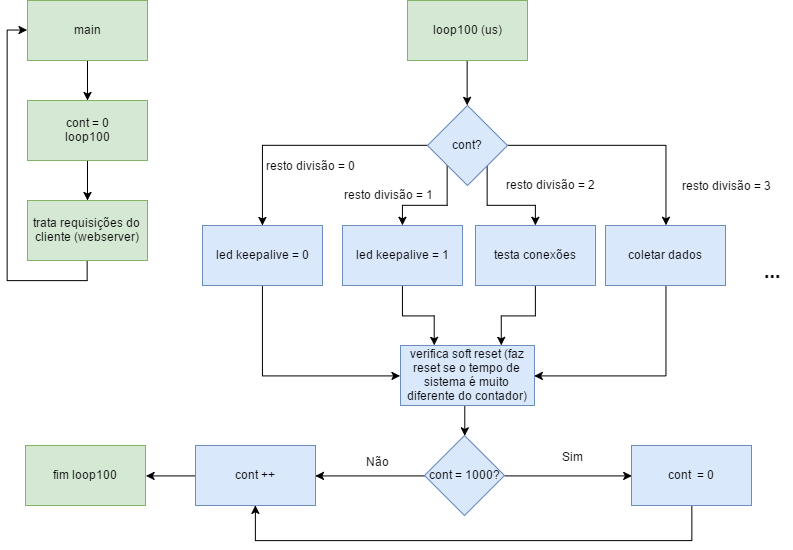
\includegraphics[width=0.8\textwidth]{rotinaMultiplexacao}
\label{fig:rotinaMultiplexacao}
\end{figure}

\subsubsection{Tratamento de indisponibilidade}
Nos casos de indisponibilidade de Internet, servidor ou rede local, o seguinte procedimento foi adotado (observe que a indisponibilidade do próprio módulo é tratada pelo circuito antitravamento):

\begin{figure}[H]
	\centering
	\caption{Tratamento de indisponibilidade de recursos}
  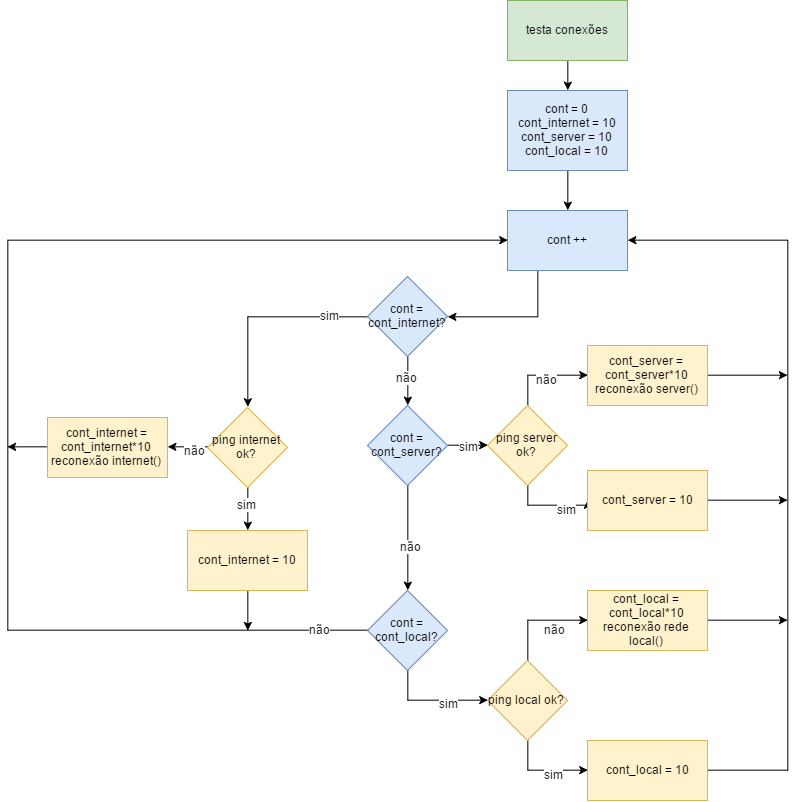
\includegraphics[width=0.8\textwidth]{tratamentoIndisponibilidade}
\label{fig:tratamentoIndisponibilidade}
\end{figure}

Com esse procedimento, as tentativas de reconexão à Internet, servidor e rede local estão segregadas e com tentativas realizadas em intervalos de tempo sucessivamente maiores. Desta forma, conseguimos gerenciar esses procedimentos, já que o nível de processamento é baixo.

\subsubsection{DoS local (\textit{Evil Twin})}
No caso de ataque de \textit{Evil Twin} - no qual uma rede mal-intencionada, usualmente aberta, usa o mesmo SSID da rede original com o objetivo de obter a senha - o sistema pode ficar indisponível até ao nível local. Módulos podem se conectar à rede mal-intencionada e ficarem somente com as funcionalidades offline, como acionamento de lâmpada por botão físico acoplado ao módulo. Outro problema é a queda da rede por interferência de radiofrequência ou outro mecanismo utilizado pelo usuário mal-intencionado para que os clientes se desconectem, tentem reconexão e forneçam a senha da rede.

Para mitigar esses riscos, os módulos executam o seguinte procedimento:

\begin{figure}[H]
	\centering
	\caption{Tratamento de ataque de DoS Local}
  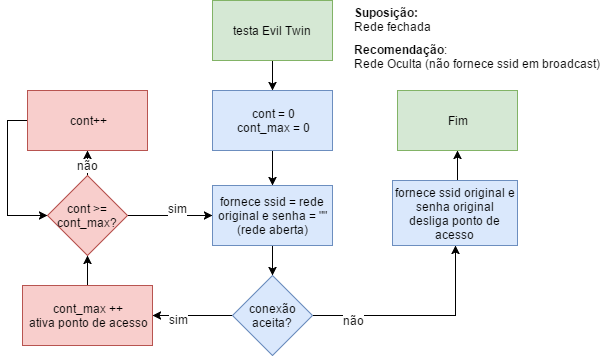
\includegraphics[width=0.8\textwidth]{tratamentoDoS}
\label{fig:tratamentoDoS}
\end{figure}

\subsubsection{Comunicação por MQTT}
Para o desenvolvimento da comunicação por MQTT com o Morpheus no módulo, foi usada a biblioteca PubSub para Arduino.

Para cada módulo existem identificador e senha, que são parâmetros próprios saídos de fábrica, além de configurações de porta e endereço do Morpheus local padrões.

O controle de comunicação foi realizado da seguinte forma:

\begin{enumerate}
	\item Só há tentativa de conexão MQTT em caso de haver conexão do Wi-Fi e o horário interno estar configurado --- caso contrário, pode-se provocar travamento do módulo ou envio de mensagens sem \emph{timestamp}.
	\item É executada configuração de \emph{callback} e de servidor MQTT a cada reconexão -- este ponto foi crítico para o bom funcionamento da comunicação.
	\item No \emph{callback} ocorre recebimento de mensagens e tratamento (\emph{parsing} da mensagem recebida, o que é feito por meio de obtenção de seu tipo e redirecionamento para rotinas específicas para obtenção dos parâmetros de interesse de cada mensagem.
	\item Envio de mensagens de estado a cada um minuto ou quando houver mudança brusca em um dos sensores (presença, abertura, umidade ou temperatura) ou então requisição de atuação; nesses casos de envio rápido, a mensagem é inserida no início da fila de saída e enviada logo em seguida, em até um segundo.
	\item Após o tratamento inicial das mensagens e a obtenção dos parâmetros de interesse, ocorre a persistência nas variáveis internas e gravação da EEPROM para que configurações e estados executados no aplicativo backup ou pela dashboard sejam refletidos dos dois lados, tornando transparente ao usuário o uso de qualquer um dos aplicativos e integrando suas funcionalidades.
	\item Ainda em fase final, após a persistência de variáveis na EEPROM, ocorre a inclusão na fila de saída de mensagens de confirmação para o servidor local.
	\item A fila de saída é usada para o envio periódico das mensagens de estado.
\end{enumerate}

\begin{figure}[H]
	\centering
	\caption{Exemplo de estado da fila de saída de mensagens MQTT do módulo}
	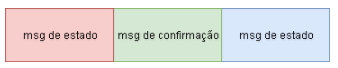
\includegraphics[width=0.5\textwidth]{filasaidaMQTT}
	\label{fig:filasaidaMQTT}
\end{figure}

Mensagens de estado periódicas (azuis) são inseridas no final da fila. No caso de acionamento, uma mensagem de estado (vermelha) é inserida no início da fila, e, em caso de configuração, uma mensagem de confirmação também é inserida no início da fila.

Por fim, vale destacar a necessidade de alteração da biblioteca PubSub para suportar mensagens maiores. Em caso de impossibilidade de envio de mensagens maiores, todo o protocolo deveria ser alterado para comportar mensagens mais compactas ou então deveria haver o uso de algum mecanismo de codificação ou compactação em conjunto com o protocolo desenvolvido.

\subsection{Diagrama}
Abaixo está o diagrama do circuito impresso (PCB).

\begin{figure}[H]
	\centering
	\caption{Diagrama PCB do Módulo Base}
  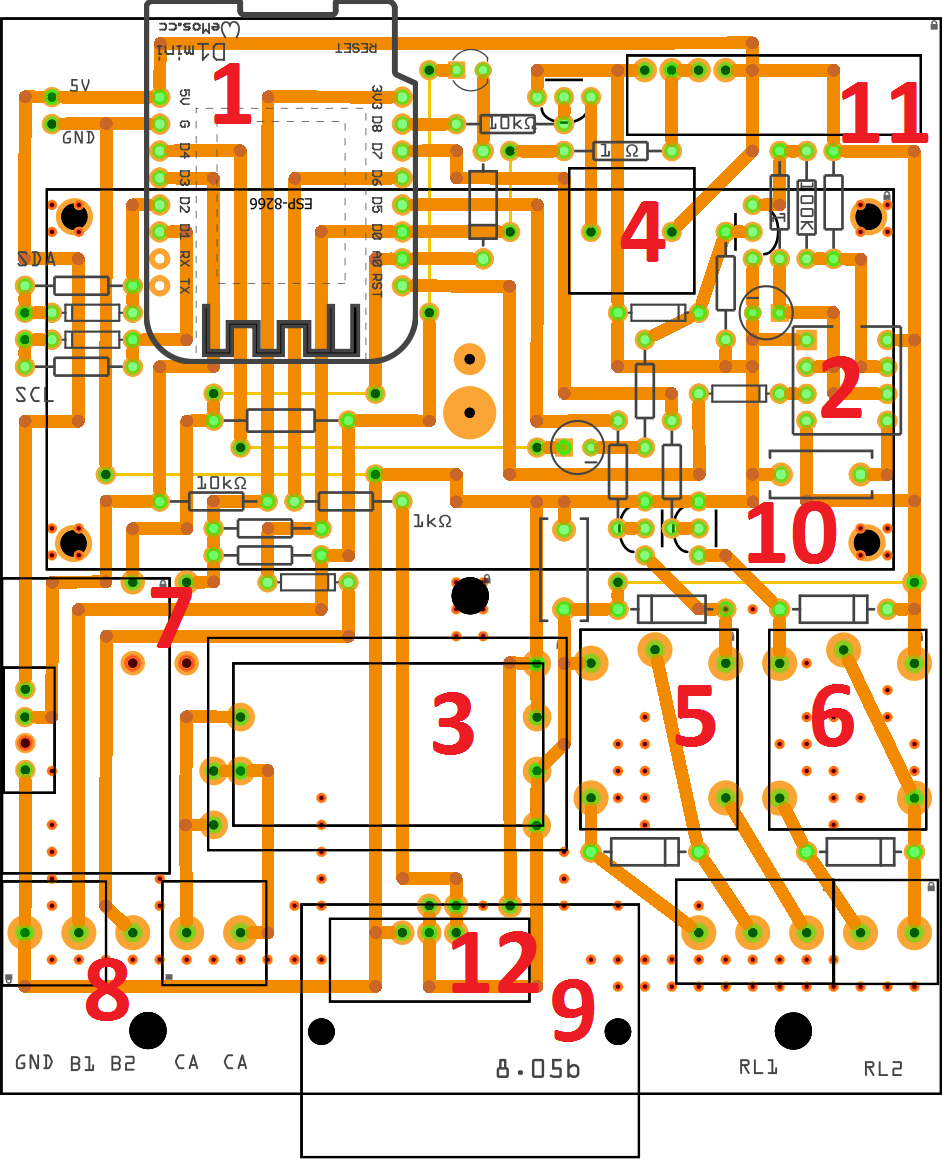
\includegraphics[width=0.8\textwidth]{diagramaModuloBase}
\label{fig:diagramaModuloBase}
\end{figure}

\begin{enumerate}
\item Wemos D1 mini
\item Astável 555
\item Fonte 5V 3W
\item \textit{Buzzer}
\item Relé 1
\item Relé 2
\item \emph{Hard reset}
\item Botões
\item Presença
\item RF-RX
\item RF-TX
\end{enumerate}

\begin{figure}[H]
	\centering
	\caption{Diagrama elétrico do Módulo Base}
  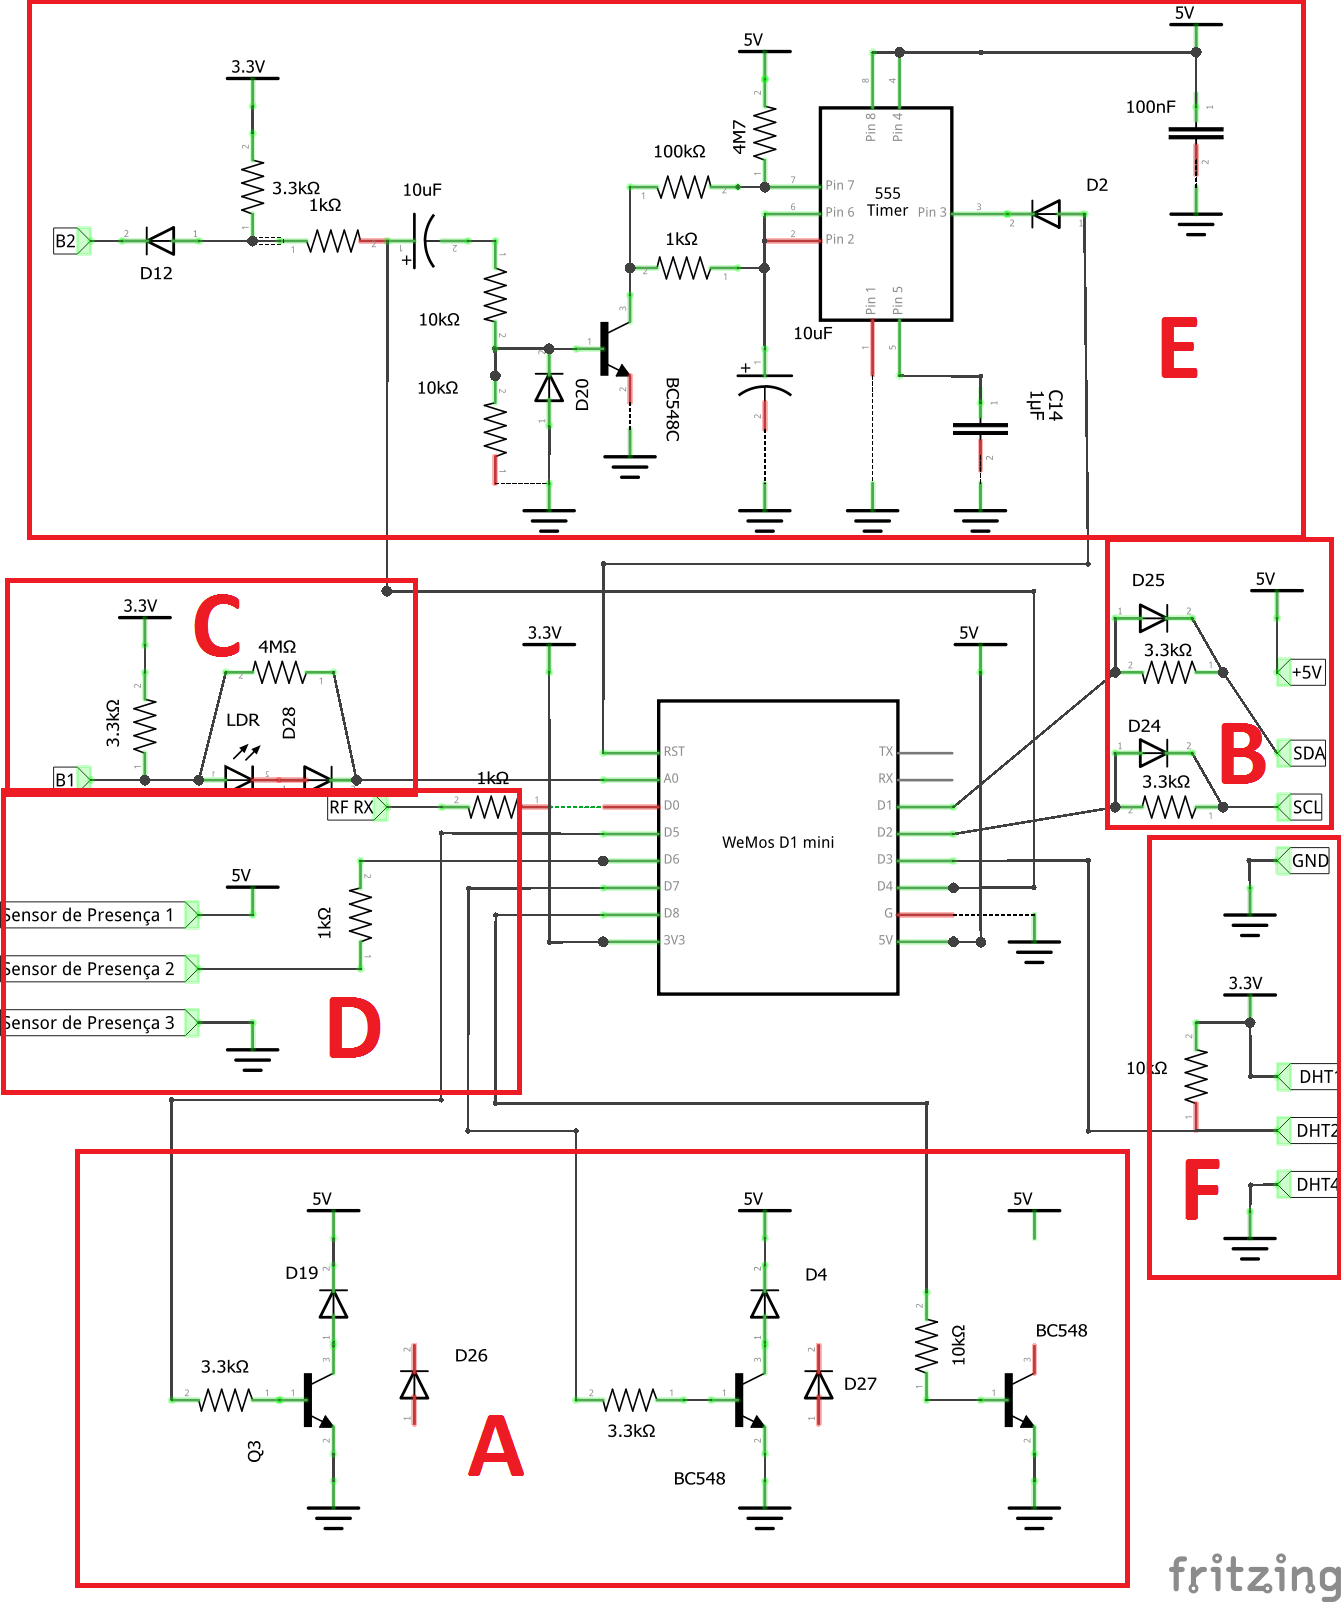
\includegraphics[width=0.8\textwidth]{esquematicoModuloBase}
\label{fig:esquematicoModuloBase}
\end{figure}

% TODO revisar as legendas desse cara, usar as letras da imagem?
\begin{description}
\item [A - Saídas] Circuitos simples de transistor para acionamento de relés (para lâmpadas) e \emph{buzzer}.
\item [Proteção 3V3 5V] Como o display trabalha com tensão de 5V, há proteções com diodos para não danificar as entradas digitais do Wemos D1 mini, que trabalha com tensão de 3V3.
\item [3 Entradas em A0] O circuito tem como entradas um botão (para acionamento do relé 1), o LDR (para chaveamento da luz de fundo do display) e um outro botão para \emph{hard reset} do dispositivo, todos em uma entrada analógica, cujo mapeamento E/S é da seguinte forma:

\begin{figure}[H]
	\centering
	\caption{Entradas em A0}
  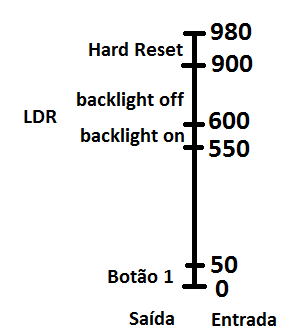
\includegraphics[width=0.4\textwidth]{entradasEmA0}
\label{fig:entradasEmA0}
\end{figure}

\item [Presença ou RF-TX] A entrada digital D6 é usada exclusivamente como entrada do sensor de presença PIR ou receptor RF.
\item [Astável 555 para \emph{hard reset} e Botão] A porta D6 é usada como LED \textit{keep alive} do módulo. Sua demora ao piscar indica que o módulo está travado ou demorando muito para processar algo, o que não deveria acontecer, uma vez que os procedimentos estão multiplexados no tempo de acordo com seus tempos limite. Dessa forma, essa saída está conectada a um circuito antitravamento, que executa o \emph{reset} nos casos mencionados, de travamento ou \textit{timeout}.

O primeiro capacitor tem como objetivo desacoplamento DC, de forma que a entrada do circuito envolvendo o astável 555 seja somente AC. Assim, permanências em 0 ou 1 indicam travamento.

Enquanto o LED pisca em intervalos esperados regularmente, o transistor conduz e mantém uma saída dente de serra muito próxima de 0. Quando o módulo trava, o transistor não conduz mais, e a saída passa a oscilar entre 1/3 e 2/3 da tensão total. Observe que o carregamento é feito pelo resistor de 4M7, muito maior que o resistor de 100k, fazendo com que o tempo de carga seja muito maior que o tempo de descarga, uma vez que esses tempos são diretamente proporcionais à constante de tempo dos circuitos RC, que é dada pelo produto do R*C. Durante a descarga, o \emph{reset} da placa é realizado. Observe que os tempos foram ajustados pelos valores dos componentes discretos, para que o tempo entre \emph{resets} sucessivos seja menor que o tempo necessário para o módulo voltar a funcionar após um \emph{reset}.

Segue abaixo uma ilustração sobre o funcionamento do circuito.

\begin{figure}[H]
	\centering
	\caption{Funcionamento do circuito antitravamento}
  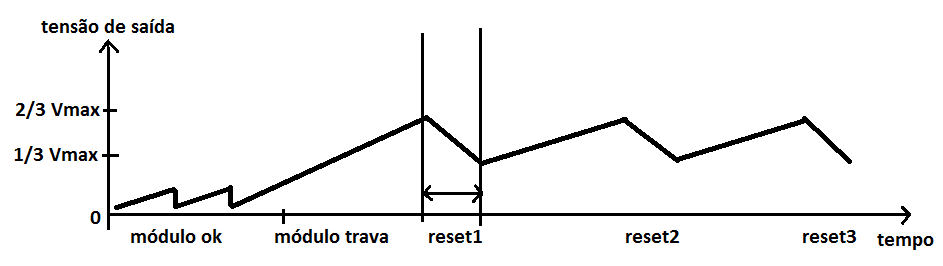
\includegraphics[width=0.8\textwidth]{circuitoAntiTravamento}
\label{fig:circuitoAntiTravamento}
\end{figure}

\item [DHT11] Entrada D3 é ligada a uma montagem básica para leitura de umidade e temperatura através do periférico DHT11.

\end{description}

\subsection {Montagem}

As fotos e comentários seguintes descrevem o processo de montagem física dos quatro módulos usados neste trabalho. Além destes, outras versões também foram construídas anteriormente no decorrer do projeto, instaladas na residência de um dos membros do grupo e usados para coleta de dados. Tais versões, por se tratarem de protótipos, não têm sua montagem completamente documentada, tampouco a uniformidade apresentada nos módulos seguintes.
Ao final, também consta o procedimento utilizado para validação dos módulos após sua construção, que contribuiu para a identificação de ligações não realizadas e outros problemas de montagem.

\begin{figure}[H]
	\centering
	\caption{Evolução do hardware (de fevereiro/17 a setembro/17)}
	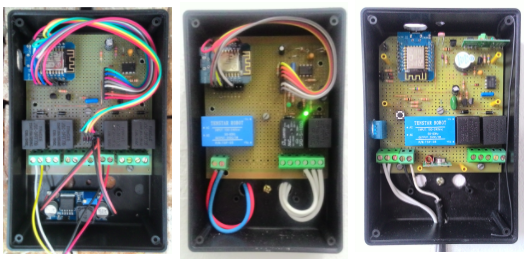
\includegraphics[width=0.8\textwidth]{evolHW}
	\label{fig:evolHW}
\end{figure}

\begin{figure}[H]
	\centering
	\caption{Evolução da caixa de proteção e display}
	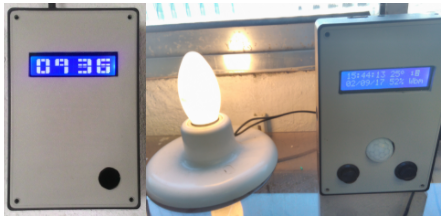
\includegraphics[width=0.8\textwidth]{evolProtDisplay}
	\label{fig:evolProtDisplay}
\end{figure}

\begin{figure}[H]
	\centering
	\caption{Materiais e preparação da placa padrão}
	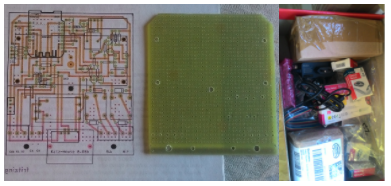
\includegraphics[width=0.8\textwidth]{materiaisPrepPlaca}
	\label{fig:materiaisPrepPlaca}
\end{figure}

\begin{enumerate}
	\item Primeiramente, a partir do esquemático em escala real, foram cortados e realizados furos na placa padrão.

	\begin{figure}[H]
		\centering
		\caption{Posicionamento dos componentes}
		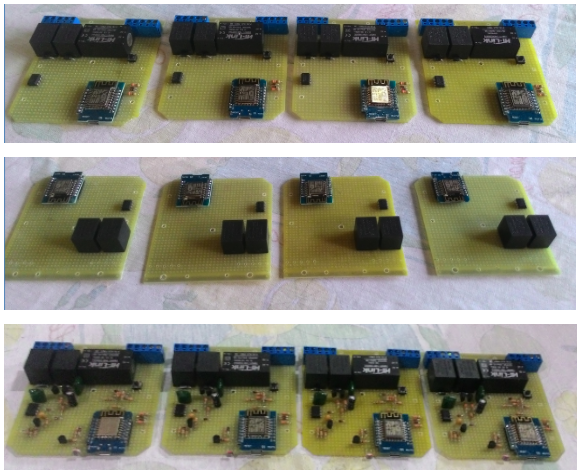
\includegraphics[width=0.8\textwidth]{PosicionamentoComp}
		\label{fig:PosicionamentoComp}
	\end{figure}

	\item Em seguida, foram posicionados os componentes.

	\begin{figure}[H]
		\centering
		\caption{Preparação dos displays com o I2C e soldagem}
		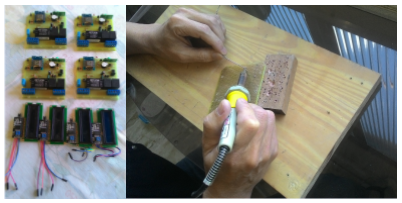
\includegraphics[width=0.8\textwidth]{PrepI2CSoldagem}
		\label{fig:PrepI2CSoldagem}
	\end{figure}

	\item A próxima etapa foi soldar as trilhas por baixo conforme o diagrama. Também foi necessário soldar o I2C com o display. Essa é a etapa mais demorada, que poderia ser facilmente operacionalizada ao serem adotadas placas de circuito impresso, o que aumentaria muito a capacidade de montagem.

	\begin{figure}[H]
		\centering
		\caption{Preparação das caixas para os módulos}
		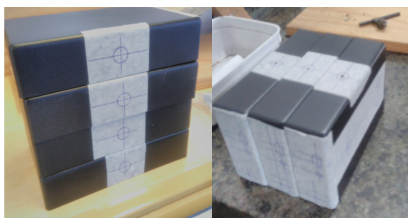
\includegraphics[width=0.8\textwidth]{PrepCaixasModulos}
		\label{fig:PrepCaixasModulos}
	\end{figure}

	\item Prossegue-se para a marcação das caixas para uso das furadeiras e lixas. Com ferramentas mais adequadas, essa etapa também poderia ser mais rápida e eficiente.

	\begin{figure}[H]
		\centering
		\caption{Caixa protetora, ligação dos botões e cabos de força}
		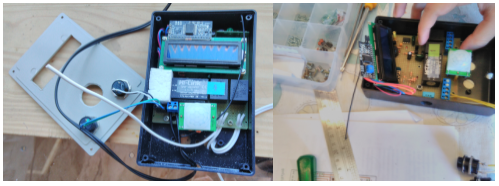
\includegraphics[width=0.8\textwidth]{BotoesCabosForca}
		\label{fig:BotoesCabosForca}
	\end{figure}

	\item Com a caixa preparada, foi possível inserir as placas padrão com os componentes e trilhas. Restou fixá-los com parafusos, montar a sustentação do display e sensor de presença (também integrado nesse passo), isopor para isolar termicamente o medidor de temperatura e umidade DHT, além de fazer as ligações dos botões, cabos de força e fios dos relés.

	\begin{figure}[H]
		\centering
		\caption{Quatro módulos prontos}
		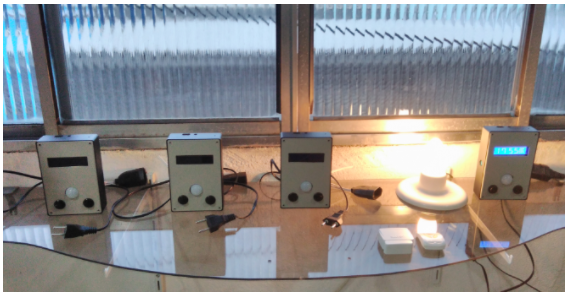
\includegraphics[width=0.8\textwidth]{QuatroModulos}
		\label{fig:QuatroModulos}
	\end{figure}

\end{enumerate}

\subsubsection {Montagem}
\begin{enumerate}
	\item Carregar programa para testar módulo;
	\item Realizar setup da conexão com a rede Wi-Fi;
	\item Verificar com o multímetro se há curto em algumas ligações principais (terra, VCC);
	\item Checar a alimentação da fonte e sua saída correta;
	\item Realizar o \emph{hard reset} ao apertar o botão atrás do isopor do DHT até ouvir 10 bipes;
	\item Fazer o passo 2 novamente, pois o módulo deve ter voltado à versão de fábrica. Logo em seguida, fazer o teste de \emph{auto reset}, que serve para verificar se o circuito antitravamento está funcionando. Para esse teste, é simulado uma pausa do sinal \emph{keep alive} que o circuito baseado no astável 555 monitora;
	\item Cobrir o sensor de presença. Verificar a inatividade no aplicativo. Descobrí-lo e verificar atividade;
	\item Executar o passo 7 para o sensor de luminosidade (LDR) também;
	\item Verificar com um medidor externo ou consulta a um site de previsões do tempo se as medidas de temperatura e umidade estão de acordo. Realizar ajuste (offset) no aplicativo se necessário;
	\item Verificar o funcionamento dos botões, acionando-os um por um;
	\item Checar o acionamento dos relés pelo aplicativo web também;
	\item Após gravar o RF de um controle para os dois relés, testar seu funcionamento;
	\item Verificar com um multímetro a saída dos relés (se troca de nível com acionamento pela página web, botões e controle RF).
\end{enumerate}
